%!LW recipe = pdflatex → biber → pdflatex (2x)
\documentclass[conference]{IEEEtran}
\IEEEoverridecommandlockouts
% The preceding line is only needed to identify funding in the first footnote. If that is unneeded, please comment it out.
%\usepackage{cite}
\usepackage{amsmath,amssymb,amsfonts}
\usepackage{algorithmic}
\usepackage{graphicx}
\usepackage{textcomp}
\usepackage{xcolor}
\usepackage{float}
\usepackage[caption=false,font=normalsize,labelfont=small,textfont=sf]{subfig}
\usepackage[font=small,aboveskip=0pt,belowskip=-15pt]{caption}
\usepackage{setspace}
\setstretch{0.95}
\usepackage[backend=biber,style=ieee,maxnames=1,doi=false,isbn=false,url=false]{biblatex}
\DeclareSourcemap{
  \maps[datatype=bibtex]{
    \map{
      \step[fieldsource=journal, match={Nature Electronics}, replace={Nat. Electron.}]
      \step[fieldsource=journal, match={Nature Communications}, replace={Nat. Commun.}]
      \step[fieldsource=journal, match={npj 2D Materials and Applications}, replace={npj 2D Mater. Appl.}]
      \step[fieldsource=journal, match={Advanced Electronic Materials}, replace={Adv. Electron. Mater.}]
      \step[fieldsource=journal, match={IEEE Transactions on Electron Devices}, replace={IEEE Trans. Electron Devices}]
      \step[fieldsource=journal, match={Nature Nanotechnology}, replace={Nat. Nanotechnol.}]
      \step[fieldsource=journal, match={Physical Review Letters}, replace={Phys. Rev. Lett.}]
    }
  }
}
\AtEveryBibitem{%
  \clearfield{pages}%
  \clearfield{month}%
  \clearfield{number}
}
\DeclareFieldFormat{journaltitle}{\iffieldundef{shortjournal}
  {#1}
  {\printfield{shortjournal}}}

\addbibresource{references.bib}

\AtBeginBibliography{%
  \setlength{\bibitemsep}{0pt}
  \setlength{\bibparsep}{0pt}
}
\AtBeginBibliography{\small}
\def\BibTeX{{\rm B\kern-.05em{\sc i\kern-.025em b}\kern-.08em
    T\kern-.1667em\lower.7ex\hbox{E}\kern-.125emX}}
    
\begin{document}

\title{Reliability Assessment of hBN-Encapsulated \\ TMD Devices: from FETs to Inverters\\
%A Comprehensive Reliability Assessment of hBN-encapsulated TMD FETs and Inverters\\
%Hysteresis and Reliability of \\ hBN-encapsulated MoS$_2$ FETs\\
\thanks{We gratefully acknowledge funding from the European Innovation Council under project number 101223249.}
}

\author{
\IEEEauthorblockN{
F. de los Santos-Prieto\IEEEauthorrefmark{1},
A. Verdianu\IEEEauthorrefmark{1},
A. Provias\IEEEauthorrefmark{1},
A. Karl\IEEEauthorrefmark{1},
L. Pettorosso\IEEEauthorrefmark{2},
D. Polyushkin\IEEEauthorrefmark{2},\\
D. Waldhoer\IEEEauthorrefmark{1},
T. Müller\IEEEauthorrefmark{2}, 
T. Grasser\IEEEauthorrefmark{1}, and 
T. Knobloch\IEEEauthorrefmark{1},
}

\IEEEauthorblockA{\IEEEauthorrefmark{1}
Institute for Microelectronics, Technical University of Vienna, Vienna, Austria
}

\IEEEauthorblockA{\IEEEauthorrefmark{2}
Institute of Photonics, Technical University of Vienna, Vienna, Austria
}

Email: \{delossa\textbar knobloch\}@iue.tuwien.ac.at
}

\maketitle

\begin{abstract}
This document is a model and instructions for \LaTeX.
This and the IEEEtran.cls file define the components of your paper [title, text, heads, etc.]. *CRITICAL: Do Not Use Symbols, Special Characters, Footnotes, 
or Math in Paper Title or Abstract.
\end{abstract}

\begin{IEEEkeywords}
component, formatting, style, styling, insert
\end{IEEEkeywords}

\section{Introduction}

As device miniaturization continues, the performance of traditional logic devices based on bulk semiconductors becomes increasingly constrained, either by the exacerbation of short-channel effects in field-effect transistors (FETs) when the channel thickness is not scaled accordingly, or by the associated mobility reduction when it is~\cite{liu_promises_2021}. To overcome this inherent trade-off of bulk channels, two-dimensional (2D) materials, whose carrier mobility exhibits weak thickness dependence, have attracted significant attention. Among them, transition-metal dichalcogenides (TMDs) offer suitable bandgaps and currently represent the backbone of active logic devices based on 2D materials, with MoS$_2$ being the most mature option for realizing n-channel FETs~\cite{das_transistors_2021}. 

However, important limitations arise with the use of 2D materials. While their dangling-bond-free interfaces mitigate the mobility drop for scaled devices, the absence of covalent bonding at the oxide–channel interface leads to increased instability compared to the well-established SiO$_2$/Si interface~\cite{lan_reliability_2025}. This instability typically originates from charge transfer and transport processes through the gate stack, manifests during device operation, and entails shifts in key device parameters (most notably the threshold voltage), thereby compromising the functionality and performance of the resulting logic circuits~\cite{mulong_luo_impacts_2015}.

To mitigate the aforementioned instabilities, different gate stack concepts and optimizations have been proposed to reduce charge transfer without compromising device performance. A promising approach involves the use of 2D insulators to achieve well-passivated interfaces with the channel, thereby enhancing device stability while enabling the construction of van der Waals heterostructures to tune device properties~\cite{geim_van_2013}. Among the candidate materials, hexagonal boron nitride (hBN) is the most ubiquitous; however, its low dielectric constant limits its use as a single insulating material in deeply scaled devices due to the expected high gate leakage~\cite{knobloch_performance_2021}. However, recent studies propose the use of hBN layers to encapsulate a bulk gate oxide, thereby improving device stability at the expense of increased fabrication complexity~\cite{piacentini_stable_2022}.

To benchmark this and other proposed approaches, it is essential to quantify the detrimental instability effects, which can be observed either under varying device conditions, as in classical hysteresis and bias temperature instability (BTI) measurements where the gate voltage is altered, or under constant conditions, as in low-frequency noise measurements. In particular, the former have proven to be straightforward and highly effective techniques for assessing device reliability~\cite{provias_reliability_2023}. However, inaccurate conclusions may be drawn if key experimental parameters and essential characteristics of the devices under test are overlooked. For instance, while the time required to perform the up- and down-sweeps in hysteresis measurements is rarely reported, it has been shown to have a significant impact on the underlying physical mechanisms of hysteresis and the resulting measurements~\cite{karl_standardized_2025}. Similarly, as the impact of most degradation mechanisms depends on insulator thickness, it becomes essential to normalize both hysteresis and BTI shifts with respect to thickness to enable accurate comparisons between samples.

In this work, a comprehensive reliability assessment of hBN-encapsulated MoS$_2$ FETs is presented, with hysteresis and BTI measurements constituting the core of the analysis and providing complementary insights. Special emphasis is placed on the number of analyzed devices to capture variability in instability behavior, as well as on key measurement parameters, such as the sweep time and the drain voltage in hysteresis measurements. The analysis is further extended to characterize depletion-load nMOS inverters based on these hBN-encapsulated FETs, enabling a straightforward evaluation of the reliability of this platform for deeply scaled logic applications. The rest of the manuscript is organized as follows: Section~\ref{sec:device} describes the device fabrication and analyzes the performance of the resulting FETs and inverters. Section~\ref{sec:hysteresis} presents a comprehensive analysis of the hysteresis behavior of the fabricated devices, while Section~\ref{sec:BTI} focuses on BTI measurements. Finally, conclusions are drawn in Section~\ref{sec:conclusions}.

\section{Device Fabrication and Performance}\label{sec:device}

\begin{figure*}[ht]
    \centering
    \subfloat[]{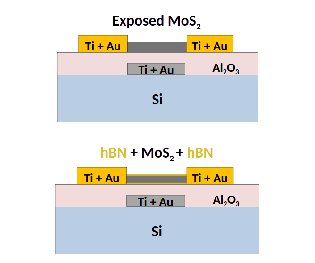
\includegraphics[]{figures/crossections.pdf}\label{fig:crosssection_exposed}} 
    \hspace{0.25in}
    \subfloat[FET A]{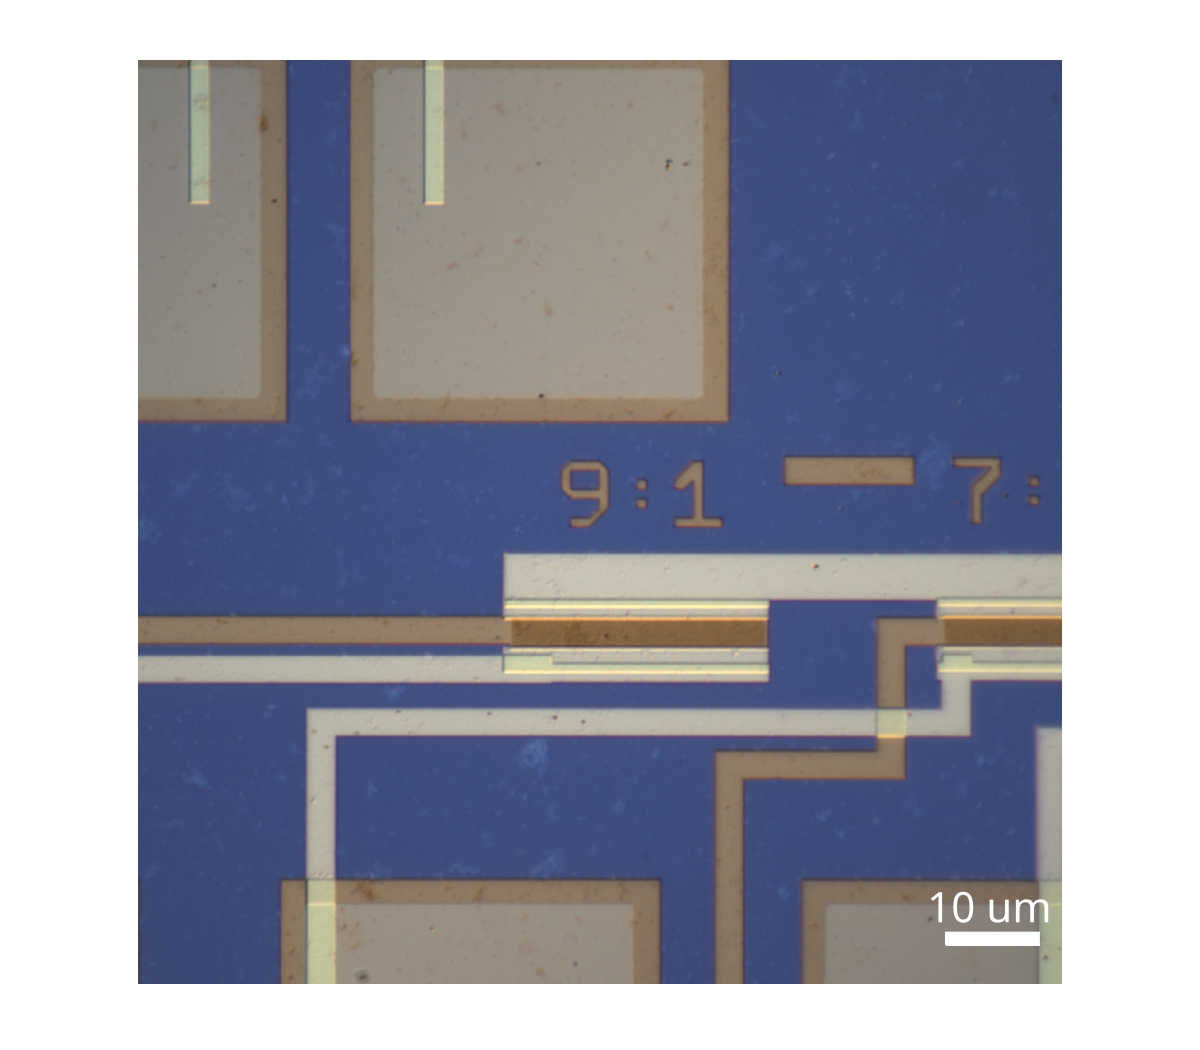
\includegraphics[]{figures/OM_FET.pdf}\label{fig:OM_hBN_FET}}
    \hfill
    \subfloat[FET A]{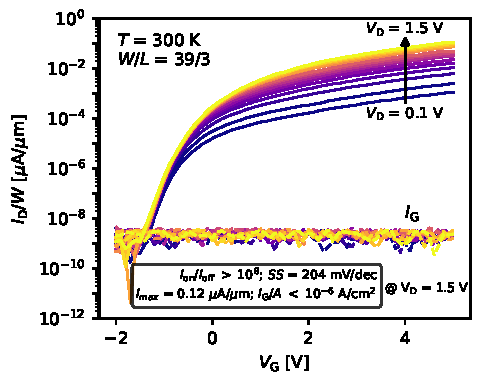
\includegraphics[]{figures/IdVg_encapsulated_1.pdf}\label{fig:performance_hbn_FET}} \\[-0.75em]
    \subfloat[\small Inverter A]{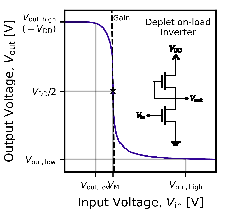
\includegraphics[]{figures/inverter_VTC_schematic.pdf}\label{fig:inverter_schematic}}
    \hspace{0.25in}
    \subfloat[\small Inverter A]{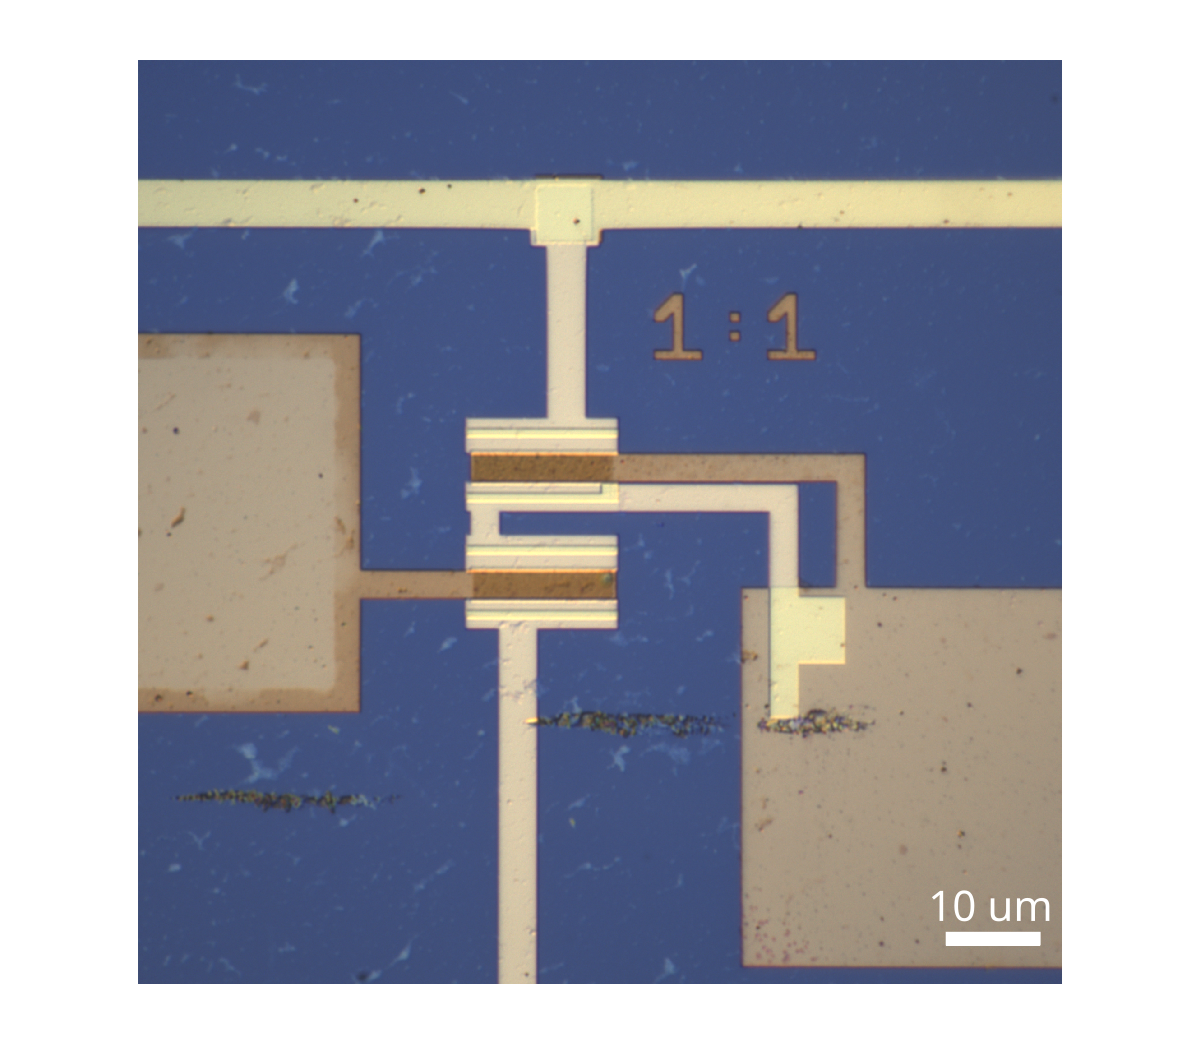
\includegraphics[]{figures/OM_INV.pdf}\label{fig:OM_hBN_INV}}
    \hfill
    \subfloat[\small Inverter A]{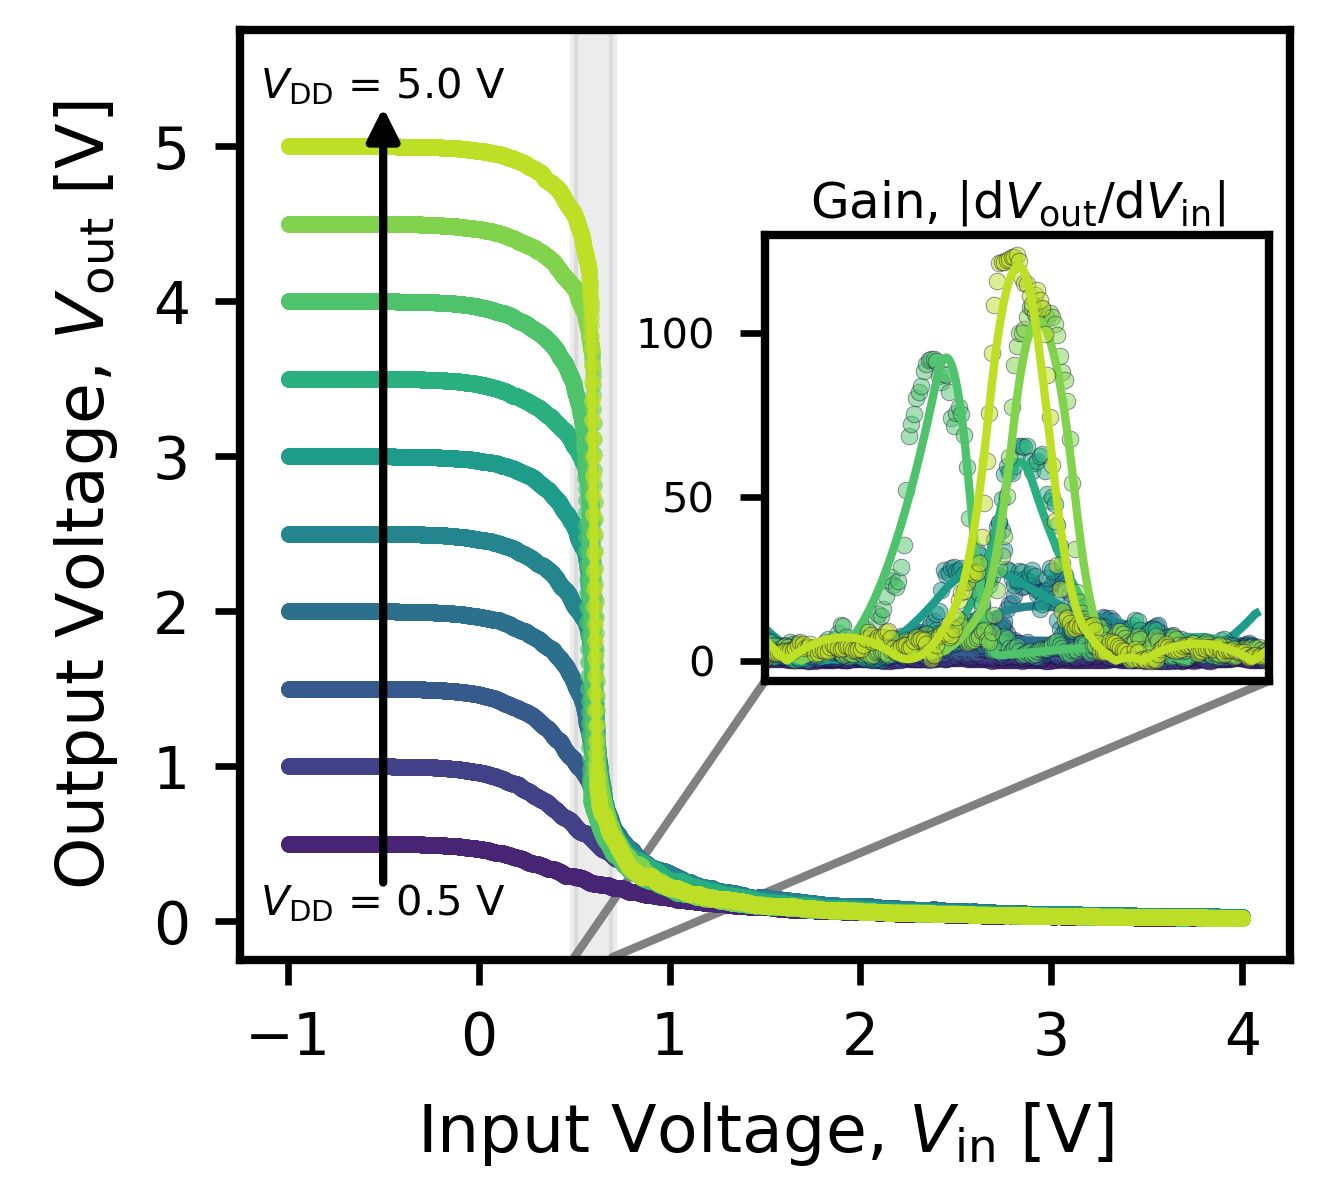
\includegraphics[]{figures/inverter_gain.png}\label{fig:inverter_gain}}
    \caption{~(a)~\textbf{Device cross-section:} Schematics of exposed (top) and hBN-encapsulated (bottom) MoS$_2$ FETs.~(b)~\textbf{FET optical image:} Fabricated hBN-encapsulated FET.~(c)~\textbf{Performance of the fabricated devices:} $I_\mathrm{D(G)}$--$V_\mathrm{G}$ curves for different drain voltages and key device metrics extracted at $V_\mathrm{D}$ = 1.5 V.~(d)~\textbf{Inverter VTC:} Typical voltage transfer curve of a depletion-load nMOS inverter. For simplicity, $V_\mathrm{M}$ is defined as the input voltage at which the output equals half the supply voltage $V_\mathsf{DD}$.~(e)~\textbf{Inverter optical image:} Fabricated hBN-encapsulated inverter.~(f)~\textbf{Inverter performance with $V_\mathsf{DD}$:} Inverter VTC curves for different supply voltages and the corresponding gain curves for the higher supply voltages.}
    \label{fig:devices_fabrication_performance}
\end{figure*}

The devices comprise a Ti/Au–Al$_2$O$_3$–MoS$_2$ gate stack and were fabricated following the approach in~\cite{polyushkin_analogue_2020}, with additional steps to enable hBN encapsulation for the encapsulated devices following the approach in~\cite{piacentini_stable_2022}. Schematics of the cross-section for both devices are shown in Fig.~\ref{fig:crosssection_exposed}. FETs with different aspect ratios ($W/L$) and depletion-load inverters with varying driver-to-load ratios ($W_d/W_l$) were designed, as shown in the optical images in Fig.~\ref{fig:OM_hBN_FET} and Fig.~\ref{fig:OM_hBN_INV}, respectively.

The performance of the hBN-encapsulated FETs is summarized in Fig.~\ref{fig:performance_hbn_FET}. The devices exhibit an excellent $I_\mathsf{on}/I_\mathsf{off}$ ratio and low gate leakage ($I_\mathsf{G}/A$), with both metrics limited by the measurement resolution, making them well suited for low-power 2D electronics. Performance metrics such as the subthreshold slope, $SS$, and the maximum current, $I_\mathsf{max}$, show non-ideal values, with the latter likely diminished by the contact resistances of the device. All FET metrics were extracted at a drain voltage of 1.5 V, in accordance with~\cite{IRDS}. The schematic of a depletion-load inverter is shown in Fig.~\ref{fig:inverter_schematic}, along with a representative experimental voltage transfer characteristic (VTC). As expected for a depletion-load design, the output high level, $V_\mathsf{out,high}$, is equal to $V_\mathrm{DD}$, whereas the output low level, $V_\mathsf{out,low}$, may deviate from the ideal value of 0 V depending on the driver-to-load ratio and the threshold voltage of the transistors. The transition point between the high and low output levels, $V_\mathrm{M}$, is defined for convenience as the input voltage at which the output equals half of the supply voltage, $V_\mathrm{DD}/2$. In Fig.~\ref{fig:inverter_gain}, the performance of an inverter with a 1/1 driver-to-load ratio is shown for different $V_\mathsf{DD}$. The inverter gain, defined as the magnitude of $dV_\mathrm{out}/dV_\mathrm{in}$ and reflecting the steepness of the transition between high and low output levels, is plotted in the inset of this figure for higher $V_\mathrm{DD}$, showing values approaching and even exceeding 100 depending on $V_\mathrm{DD}$. 

\section{Hysteresis Characterization}\label{sec:hysteresis}

\begin{figure*}[ht]
    \centering
    \subfloat[\small FET A]{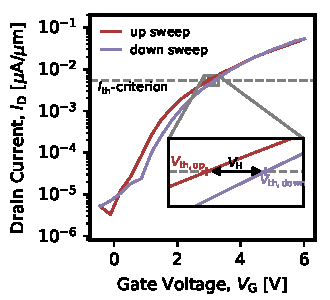
\includegraphics[]{figures/hysteresis_IdVg_example.pdf}\label{fig:example_hyst_IdVg}}
    \subfloat[\small FET A]{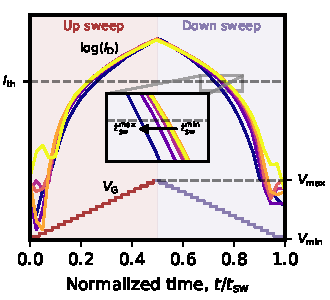
\includegraphics[]{figures/hysteresis_time_example.pdf}\label{fig:hysteresis_vs_time}}
    \hfill
    \subfloat[\small FET A]{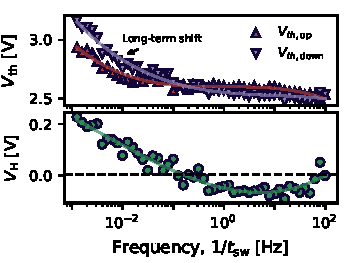
\includegraphics[]{figures/hysteresis_Vth_DeltaVth_vs_freq.pdf}\label{fig:hysteresis_vs_freq}} \\[-1.2em]
    \subfloat[\small FETs B, C]{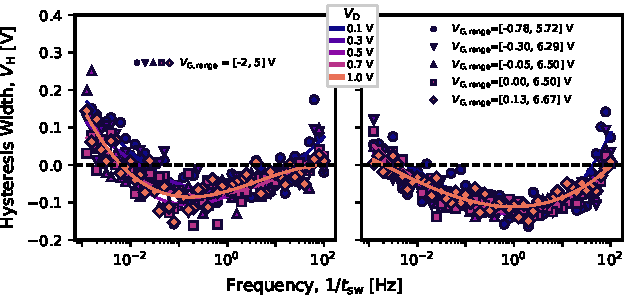
\includegraphics[]{figures/hysteresis_DeltaVth_vs_freq_differentVd.pdf}\label{fig:hyst_differentVd}}
    \hfill
    \subfloat[\small FETs D, E(enc.), $\alpha, \beta, \gamma, \delta$(non-enc.)]{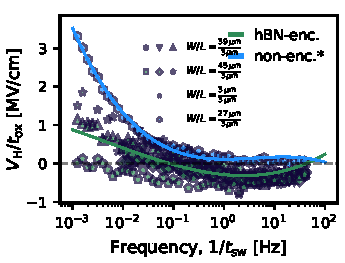
\includegraphics[]{figures/hysteresis_DeltaVth_vs_freq_comparison.pdf}\label{fig:hyst_comparison}} 
    \caption{(a) \textbf{Typical hysteresis curve}: the hysteresis width, $V_\mathsf{H}$, is defined as the difference between the threshold voltages extracted during the up and down sweeps, i.e., $V_{H} = V_\mathsf{th,up} - V_\mathsf{th,down}$ evaluated at a constant current criterion $I_\mathsf{th}$. (b) \textbf{Hysteresis dependence on the gate voltage sweep rate}: $\log(I_{D})$ and $V_\mathsf{G}$ are shown as a function of the normalized sweep time, $t/t_\mathsf{sw}$, for different sweep times, $t_\mathsf{sw}$. (c) \textbf{Hysteresis-$1/t_\mathsf{sw}$ curves}: Threshold voltages, $V_\mathsf{th,up}$ and $V_\mathsf{th,down}$, and hysteresis width, $V_\mathsf{H}$, are shown as a function of the sweep frequency, $1/t_\mathsf{sw}$. (d) \textbf{Hysteresis for varying $V_\mathsf{D}$}: The hysteresis is independent of the applied drain bias, as evaluated on two different devices. More consistent hysteresis results are obtained when using an adaptive scheme for the gate-voltage range that targets the same overdrive and the same sweep range in the subthreshold regime (right), as compared to a fixed gate-voltage range (left). (e) \textbf{Hysteresis in encapsulated vs. non-encapsulated devices}: The hysteresis width in encapsulated devices is negative (counter-clockwise), whereas in non-encapsulated devices it was of a similar magnitude but positive (clockwise) evaluated at $V_\mathsf{D}$= 0.1 V.}
    \label{fig:hysteresis}
\end{figure*}

Hysteresis measurements are a widely used method to benchmark the stability of FETs, as near-negligible hysteresis is a key prerequisite for reliable performance in digital applications. However, transistors based on 2D semiconductors such as MoS$_2$ FETs often exhibit excessive hysteresis, which can limit their practical use. Fig.~\ref{fig:example_hyst_IdVg} depicts a typical hysteresis curve in which the $I_\mathrm{D}$--$V_\mathrm{G}$ characteristics corresponding to the up and down sweeps differ from each other. This divergence can be quantified through the hysteresis width, $V_\mathsf{H}$, defined here as the difference in the threshold voltage of the transistor during the up and down sweeps, i.e., $V_\mathsf{th,up} - V_\mathsf{th,down}$\footnote{According to this definition, clockwise hysteresis corresponds to positive values of $V_\mathsf{H}$, whereas counter-clockwise hysteresis leads to negative values.}. Different techniques can be used to extract the threshold voltage; for simplicity, the constant-current criterion is adopted here. This method defines the threshold voltage as the gate voltage at which the drain current reaches a specified reference value, $I_\mathsf{th}$. Typical values of $I_\mathsf{th}$ are on the order of $10^{-7},\mathrm{A}\cdot W/L$ for bulk semiconductor devices, whereas lower values, around $10^{-9},\mathrm{A}\cdot W/L$, are more appropriate for 2D devices. In this work, the latter value is adopted.

Several measurement parameters can influence the outcome of hysteresis measurements. Fig.~\ref{fig:hysteresis_vs_time} shows the gate voltage up and down sweeps and the corresponding hysteresis curves as a function of normalized measurement time for different total sweep times, $t_\mathsf{sw}$. It can be observed that the choice of $t_\mathsf{sw}$ significantly affects the extracted threshold voltages, and consequently, the hysteresis width. In Fig.~\ref{fig:hysteresis_vs_freq}, $V_\mathsf{th,up}$, $V_\mathsf{th,down}$, and $V_\mathsf{H}$ are plotted as a function of the sweep frequency, $1/t_\mathsf{sw}$, with measurements performed from high to low frequencies. For low frequencies, a drift of the threshold voltage toward more positive values and an increase in the hysteresis width are observed, in agreement with the typical behavior of n-channel FETs under long-term positive BTI stress. However, at high frequencies, counterclockwise hysteresis is observed, as indicated by negative values of $V_\mathsf{H}$. This behavior is likely due to charge transport by mobile ions in the insulator, as other sources of counterclockwise hysteresis, such as ferroelectricity, can be ruled out~\cite{karl_standardized_2025}.

Besides the sweep time, other important parameters are the minimum and maximum voltages reached during the sweep, i.e., the gate-voltage range, $V_\mathsf{G, range} = [V_\mathsf{min}, V_\mathsf{max}]$, as they determine the average electric field applied to the gate stack. As most of the physical mechanisms underlying hysteresis depend on the electric field, this range is expected to affect the extracted hysteresis. Another parameter that is often overlooked is the drain voltage, $V_\mathsf{D}$. On one hand, as $V_\mathsf{D}$ determines the longitudinal electric field in the device, it must be kept within a safe range to avoid interface degradation due to hot-carrier effects (a phenomenon that is still not well understood in 2D FETs). On the other hand, $V_\mathsf{D}$ may influence hysteresis measurements more subtly through its impact on the current when the threshold voltage and hysteresis width are extracted using a constant-current criterion.

Fig.~\ref{fig:hyst_differentVd} shows the impact of both $V_\mathsf{G,range}$ and $V_\mathsf{D}$ on hysteresis. In the right plot, successive hysteresis measurements are carried out at different $V_\mathsf{D}$ while keeping $V_\mathsf{G,range}$ constant on the same device. In contrast, in the left plot, the same procedure is repeated, but with $V_\mathsf{G,range}$ adapted to account for the degradation in the previous measurements. As expected, better overlap between the different measurements is observed when the adaptive scheme is employed. In both cases, no dependence on $V_\mathsf{D}$ is observed, which provides a useful sanity check that the stability of the gate stack is being probed.

Fig.~\ref{fig:hyst_comparison} provides a comparison of the hysteresis in hBN-encapsulated and non-encapsulated devices. Similar hysteresis magnitudes are observed in the samples, but with opposite sign. This suggests that the counter-clockwise hysteresis is linked to the additional fabrication steps associated with the encapsulation process.

\section{Bias Temperature Instability}\label{sec:BTI}

\begin{figure*}[ht]
    \centering
    \subfloat[\small FETs F, G]{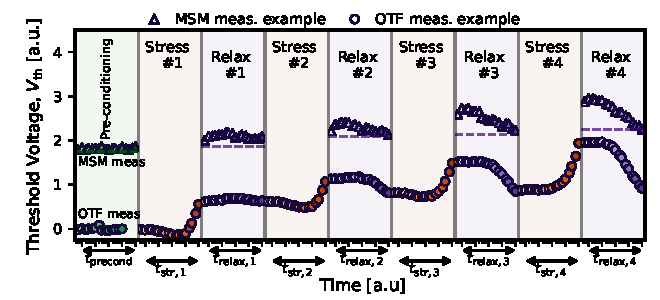
\includegraphics[]{figures/BTI_stress_time.pdf}\label{fig:OTF_MSM_time}}
    \hfill
    \subfloat[\small FET G]{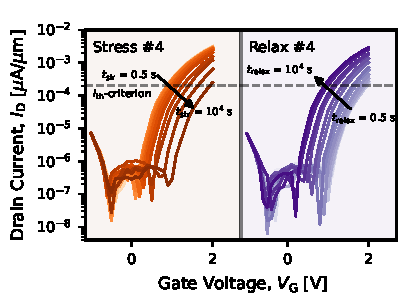
\includegraphics[]{figures/BTI_IdVg_stressrelax.pdf}\label{fig:BTI_IdVg}}
    \hfill
    \subfloat[\small FET G]{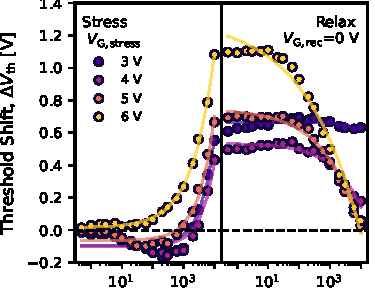
\includegraphics[]{figures/OTF_DeltaVth_strrec_differentVstr.pdf}\label{fig:OTF_differentVstr}}
    \\[-1em]
    \subfloat[\small FETs F,H,I,J,K,L]{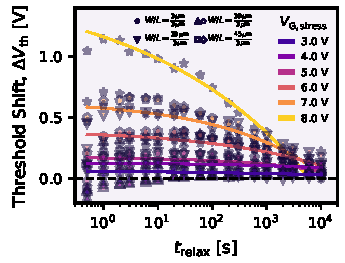
\includegraphics[]{figures/MSM_DeltaVth_duts.pdf}\label{fig:MSM_duts}}
    \hfill
    \subfloat[\small FETs F,H,I,J,K,L (enc.), $\epsilon$ (non-enc.)]{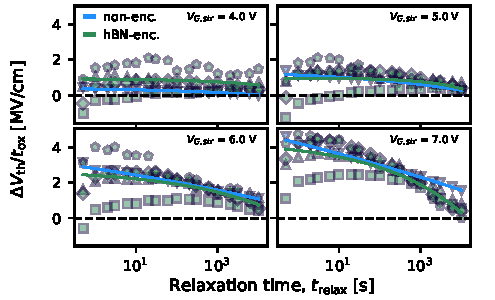
\includegraphics[]{figures/MSM_DeltaVth_comparison.pdf}\label{fig:MSM_comparison}}
    \hfill
    \subfloat[\small Inverter B]{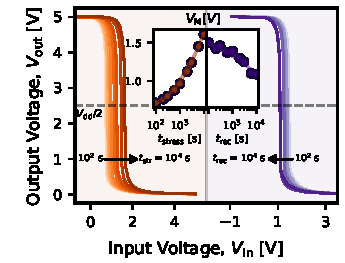
\includegraphics[]{figures/BTI_inv_stressrelax.pdf}} 
    \caption{(a)~\textbf{Types BTI experiments}: The device under test undergoes alternating periods of stress and relaxation bias conditions. Each point in the plot corresponds to the threshold voltage extracted from an $I_\mathsf{D}$--$V_\mathsf{G}$ curve at the corresponding time. Depending on the nature of the experiment, the device state is only assessed during the relaxation period in MSM measurements, whereas in OTF measurements it is continuously monitored.~(b)~\textbf{Stress and Relaxation $I_\mathsf{D}$--$V_\mathsf{G}$ curves}: The evolution of the device transfer curve during the stress and relaxation periods indicates that the degradation manifests mainly as a threshold voltage shift. Similarly to the hysteresis case, a constant-current criterion, $I_\mathsf{th}$, must be defined to extract the threshold voltage.~(c)~\textbf{OTF PBTI measurement}: Stress and relaxation curves at different stress voltages for the same device. An anomalous behavior (negative $\Delta V_\mathsf{th}$ in PBTI for n-channel FETs) is observed at lower stress voltages and relatively short times.~(d)~\textbf{MSM PBTI measurements}: Relaxation curves after 100 s at different stress voltages for six different devices. Similar degradation values and high device-to-device variations are observed at lower stress voltages.~(e)~\textbf{PBTI in encapsulated vs. non-encapsulated devices}: hBN encapsulation slightly improves resilience to PBTI stress, likely associated with the presence of an anomalous component in these devices.~(f)~\textbf{PBTI impact on inverter}: Similarly to the FET case, applying a positive bias shifts the inverter transfer curve toward higher input voltages, increasing the transition point $V_\mathsf{M}$.}
    \label{fig:BTI}
\end{figure*}

Complementary to hysteresis, positive bias temperature instability (PBTI) measurements provide an additional means to assess device reliability. Since, in contrast to hysteresis, no sweep of the gate bias is involved, high biases can be applied over prolonged periods, thereby intensifying the main instability mechanisms and probing the device long-term degradation. Fig.~\ref{fig:OTF_MSM_time} depicts the two types of BTI experiments carried out in this work: on-the-fly (OTF) and measure-stress-measure (MSM). Both approaches employ alternating periods of stress (high positive gate bias, $V_\mathsf{G,str}$) and relaxation (subthreshold gate bias, $V_\mathsf{G,relax}$) to analyze the degradation and subsequent recovery of the device characteristics over time. While in MSM experiments the device state is only assessed before and after the stress (relaxation) periods, OTF measurements monitor the device continuously throughout the entire experiment, with the device state typically evaluated through an $I_\mathsf{D}$--$V_\mathsf{G}$ measurement. If degradation and relaxation primarily manifest as a shift in the transfer curve (as shown in Fig.~\ref{fig:BTI_IdVg}), the threshold voltage can be extracted using the constant current criterion introduced in the previous section, and its difference with respect to the initial value, $\Delta V_\mathsf{th}$, can be used as the parameter to monitor degradation.

Fig.~\ref{fig:OTF_differentVstr} shows an OTF PBTI measurement in which the stress bias is consecutively increased from 3 V to 6 V across successive stress–relaxation periods. During the stress period, a negative shift of the threshold voltage is observed for times up to $10^3$ s at the first three $V_\mathsf{G,str}$ values. This negative contribution is in good agreement with the previously observed counter-clockwise hysteresis at high frequencies. The relaxation measurements show that the induced degradation becomes increasingly recoverable as the stress voltage increases, being almost fully recoverable at the two highest voltages. Fig.~\ref{fig:MSM_duts} shows MSM results for different stress biases across devices. The average degradation at low $V_\mathsf{G,str}$ is quite similar, with strong device-to-device variations. 

In Fig.~\ref{fig:MSM_comparison}, a comparison of the PBTI effect between hBN-encapsulated and non-encapsulated devices is presented through MSM measurements. In general, the encapsulated devices exhibit greater tolerance to BTI degradation. However, this apparent robustness may be partly due to the previously observed negative contribution, resulting in an overall reduction in the measured shift. Finally, Fig.~\ref{fig:OM_hBN_INV} shows the inverter behavior under PBTI stress and relaxation periods. A shift of the inverter VTC toward more positive voltages is observed, followed by a corresponding recovery in the opposite direction.

\section{Conclusions}\label{sec:conclusions}
The reliability of hBN-encapsulated MoS$_2$ devices is studied extensively through complementary hysteresis and PBTI analysis, with special attention to the choice of experimental parameters. These devices exhibit anomalous behavior in both hysteresis and BTI measurements, with negative values for the threshold voltage shifts. The origin of this anomalous behavior appears to be related to the additional fabrication steps involved in the encapsulation process, as none of the non-encapsulated devices exhibit this effect. Although the negative contribution can partially compensate for the degradation induced by a positive bias in some cases, it is far from an appropriate countermeasure, as it stems from an additional and uncontrolled physical mechanism that may compromise device stability.

\printbibliography

%\section*{References}
% \begin{thebibliography}{00}
% \bibitem{b1} G. Eason, B. Noble, and I. N. Sneddon, ``On certain integrals of Lipschitz-Hankel type involving products of Bessel functions,'' Phil. Trans. Roy. Soc. London, vol. A247, pp. 529--551, April 1955.
% \bibitem{b2} J. Clerk Maxwell, A Treatise on Electricity and Magnetism, 3rd ed., vol. 2. Oxford: Clarendon, 1892, pp.68--73.
% \bibitem{b3} I. S. Jacobs and C. P. Bean, ``Fine particles, thin films and exchange anisotropy,'' in Magnetism, vol. III, G. T. Rado and H. Suhl, Eds. New York: Academic, 1963, pp. 271--350.
% \bibitem{b4} K. Elissa, ``Title of paper if known,'' unpublished.
% \bibitem{b5} R. Nicole, ``Title of paper with only first word capitalized,'' J. Name Stand. Abbrev., in press.
% \bibitem{b6} Y. Yorozu, M. Hirano, K. Oka, and Y. Tagawa, ``Electron spectroscopy studies on magneto-optical media and plastic substrate interface,'' IEEE Transl. J. Magn. Japan, vol. 2, pp. 740--741, August 1987 [Digests 9th Annual Conf. Magnetics Japan, p. 301, 1982].
% \bibitem{b7} M. Young, The Technical Writer's Handbook. Mill Valley, CA: University Science, 1989.
% \end{thebibliography}

\end{document}
